\section{ASCbase::hphob\_\-point\_\-t Class Reference}
\label{classASCbase_1_1hphob__point__t}\index{ASCbase::hphob_point_t@{ASCbase::hphob\_\-point\_\-t}}
{\tt \#include $<$hphob\_\-point\_\-t.H$>$}

Inheritance diagram for ASCbase::hphob\_\-point\_\-t::\begin{figure}[H]
\begin{center}
\leavevmode
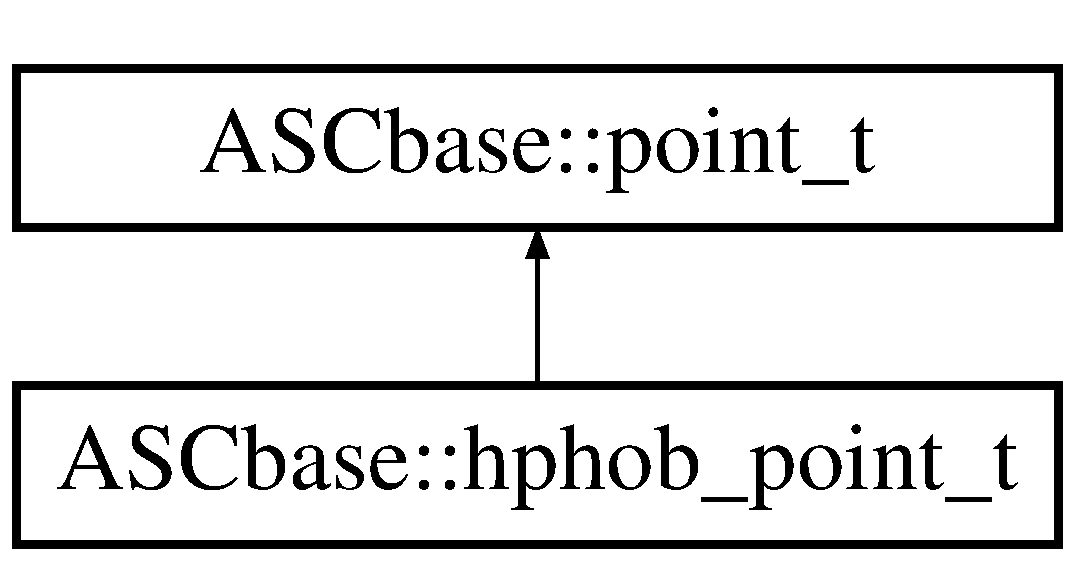
\includegraphics[height=2cm]{classASCbase_1_1hphob__point__t}
\end{center}
\end{figure}
\subsection*{Public Member Functions}
\begin{CompactItemize}
\item 
\textbf{hphob\_\-point\_\-t} (alloc\_\-t a=ALLOC\_\-POSITION)\label{classASCbase_1_1hphob__point__t_e907314b41882b3cb7ba2dee30adb580}

\item 
\textbf{hphob\_\-point\_\-t} (const \bf{hphob\_\-point\_\-t} \&p)\label{classASCbase_1_1hphob__point__t_d1a8e06a18c252ac60c2c5ed9de1b312}

\end{CompactItemize}
\subsection*{Public Attributes}
\begin{CompactItemize}
\item 
std::list$<$ atom\_\-vci $>$ \bf{atoms}\label{classASCbase_1_1hphob__point__t_7e1d90b210cbfb29b6e5fce0cecdd4d8}

\begin{CompactList}\small\item\em Protein heavy atoms that could interact. \item\end{CompactList}\end{CompactItemize}


\subsection{Detailed Description}
Use the base classes position as the computed center \char`\"{}ideal\char`\"{} template points. 



The documentation for this class was generated from the following file:\begin{CompactItemize}
\item 
hphob\_\-point\_\-t.H\end{CompactItemize}
